\section{Примеры работы}


\subsection{Примеры кодирования}


\subsubsection*{Пример кодирования 1}

Входная строка: \textit{It's easy to quit smoking. I've done it hundreds of times.}

Пример выполнения представлен на рис. \ref{fig:encode_example_1}

\begin{figure}[H]
    \centering
    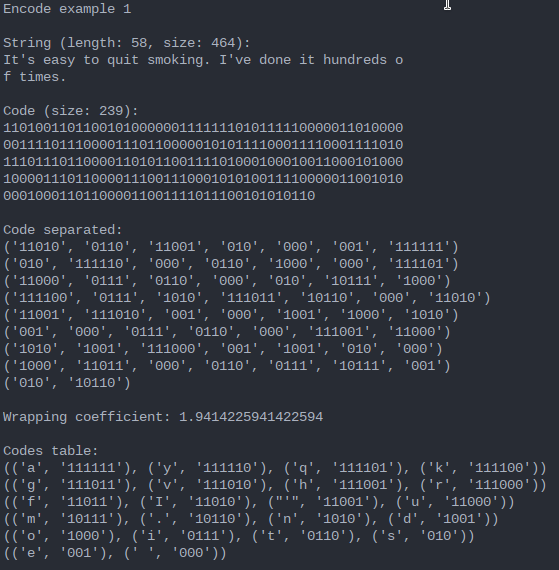
\includegraphics[width=0.7\linewidth]{photo/encode_example_1}
    \caption{Пример кодирования строки 1}
    \label{fig:encode_example_1}
\end{figure}

\subsubsection*{Пример кодирования 2}

Входная строка: \textit{Many of life's failures are people who did not realize how close they were to success when they gave up.}

Пример выполнения представлен на рис. \ref{fig:encode_example_2}

\begin{figure}[H]
    \centering
    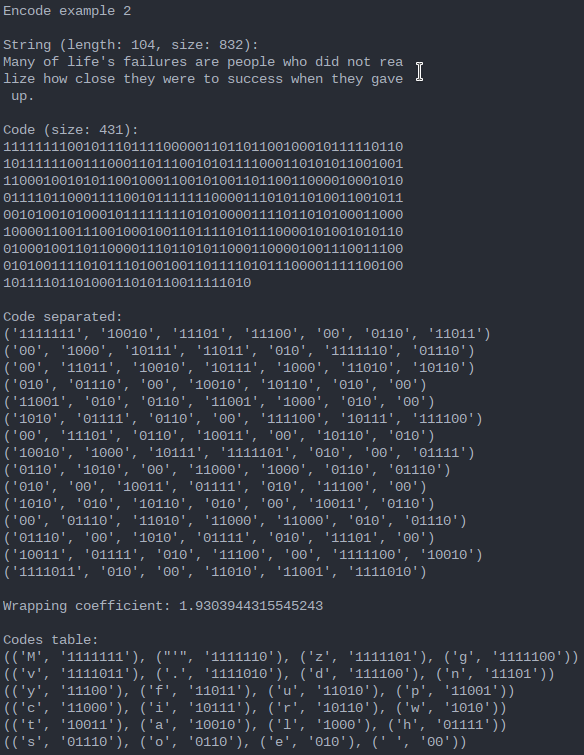
\includegraphics[width=0.7\linewidth]{photo/encode_example_2}
    \caption{Пример кодирования строки 2}
    \label{fig:encode_example_2}
\end{figure}

\subsubsection*{Пример кодирования 3}

Входная строка: \textit{May the force be with you}

Пример выполнения представлен на рис. \ref{fig:encode_example_3}

\begin{figure}[H]
    \centering
    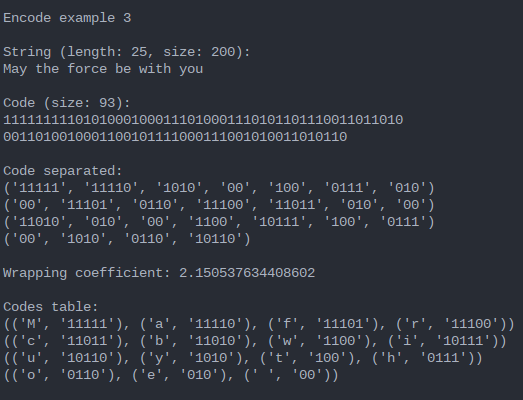
\includegraphics[width=0.7\linewidth]{photo/encode_example_3}
    \caption{Пример кодирования строки 3}
    \label{fig:encode_example_3}
\end{figure}


\subsection{Примеры декодирования}


\subsubsection*{Пример декодирования 1}

Входной код:\\ 
\textit{
01111111100010001000100011110000111110010011000100\\
1111011001100101
}

Входная таблица кодов:\\ 
\begin{lstlisting}
{
    "h": "11111",
    "a": "11110",
    "e": "1110",
    "r": "1101",
    "n": "1100",
    "g": "101",
    "i": "100",
    "t": "011",
    "s": "010",
    " ": "00"
}
\end{lstlisting}

Пример выполнения представлен на рис. \ref{fig:decode_example_1}

\begin{figure}[H]
    \centering
    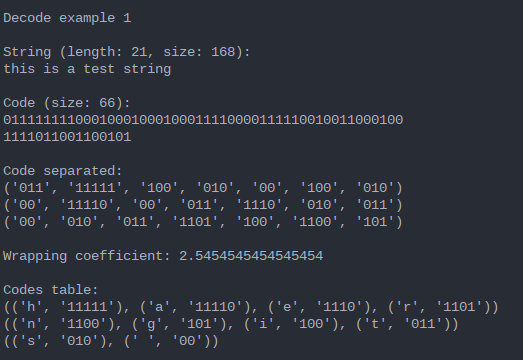
\includegraphics[width=0.7\linewidth]{photo/decode_example_1}
    \caption{Пример декодирования строки 1}
    \label{fig:decode_example_1}
\end{figure}

\subsubsection*{Пример декодирования 2}

Входной код:\\ 
\textit{
11111111010001000010101111111100011011001101010100\\
10010111000110011000100101110110111101000001111100\\
11101111000010101100100110100011101010110011100001\\
10010111001001000011110101110001101000001000010111\\
10010010101011111001101011000000011010001101110011\\
10110
}

Входная таблица кодов:\\ 
\begin{lstlisting}
{
    "T": "111111",
    "v": "111110",
    ",": "111101",
    "x": "111100",
    "p": "111011",
    "o": "111010",
    "k": "111001",
    "c": "111000",
    "m": "110111",
    ".": "110110",
    "h": "11010",
    "f": "11001",
    "l": "11000",
    "d": "10111",
    "n": "10110",
    "u": "1010",
    "r": "1001",
    "i": "1000",
    "s": "0111",
    "t": "0110",
    "a": "010",
    "e": "001",
    " ": "000"
}
\end{lstlisting}

Пример выполнения представлен на рис. \ref{fig:decode_example_2}

\begin{figure}[H]
    \centering
    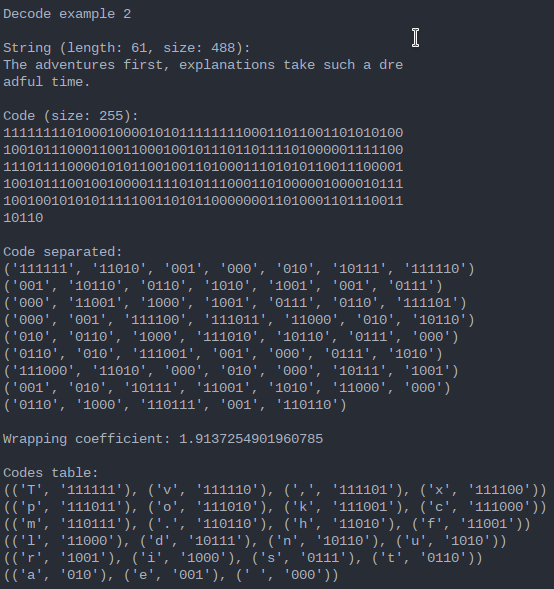
\includegraphics[width=0.7\linewidth]{photo/decode_example_2}
    \caption{Пример декодирования строки 2}
    \label{fig:decode_example_2}
\end{figure}

\subsubsection*{Пример декодирования 3}

Входной код:\\ 
\textit{
11111111001011101110101001000011111001010101001111\\
01110110111001011010111010101000011101000110100101\\
10001100110011000110100101100001110001000011101000\\
1101101110110
}

Входная таблица кодов:\\ 
\begin{lstlisting}
{
    "S": "111111",
    "d": "111110",
    "n": "11110",
    "'": "111011",
    "m": "111010",
    "g": "11100",
    "i": "11011",
    "y": "11010",
    "u": "1100",
    "c": "1011",
    "e": "1010",
    "s": "100",
    "t": "0111",
    ".": "0110",
    "o": "010",
    " ": "00"
}
\end{lstlisting}

Пример выполнения представлен на рис. \ref{fig:decode_example_3}

\begin{figure}[H]
    \centering
    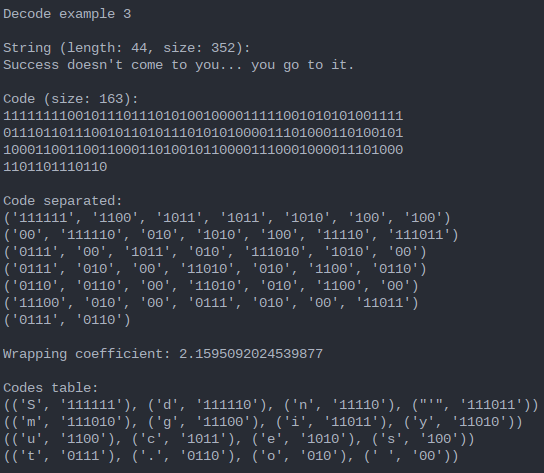
\includegraphics[width=0.7\linewidth]{photo/decode_example_3}
    \caption{Пример декодирования строки 3}
    \label{fig:decode_example_3}
\end{figure}

